
% Default to the notebook output style

    


% Inherit from the specified cell style.




    
\documentclass[11pt]{article}

    
    
    \usepackage[T1]{fontenc}
    % Nicer default font (+ math font) than Computer Modern for most use cases
    \usepackage{mathpazo}

    % Basic figure setup, for now with no caption control since it's done
    % automatically by Pandoc (which extracts ![](path) syntax from Markdown).
    \usepackage{graphicx}
    % We will generate all images so they have a width \maxwidth. This means
    % that they will get their normal width if they fit onto the page, but
    % are scaled down if they would overflow the margins.
    \makeatletter
    \def\maxwidth{\ifdim\Gin@nat@width>\linewidth\linewidth
    \else\Gin@nat@width\fi}
    \makeatother
    \let\Oldincludegraphics\includegraphics
    % Set max figure width to be 80% of text width, for now hardcoded.
    \renewcommand{\includegraphics}[1]{\Oldincludegraphics[width=.8\maxwidth]{#1}}
    % Ensure that by default, figures have no caption (until we provide a
    % proper Figure object with a Caption API and a way to capture that
    % in the conversion process - todo).
    \usepackage{caption}
    \DeclareCaptionLabelFormat{nolabel}{}
    \captionsetup{labelformat=nolabel}

    \usepackage{adjustbox} % Used to constrain images to a maximum size 
    \usepackage{xcolor} % Allow colors to be defined
    \usepackage{enumerate} % Needed for markdown enumerations to work
    \usepackage{geometry} % Used to adjust the document margins
    \usepackage{amsmath} % Equations
    \usepackage{amssymb} % Equations
    \usepackage{textcomp} % defines textquotesingle
    % Hack from http://tex.stackexchange.com/a/47451/13684:
    \AtBeginDocument{%
        \def\PYZsq{\textquotesingle}% Upright quotes in Pygmentized code
    }
    \usepackage{upquote} % Upright quotes for verbatim code
    \usepackage{eurosym} % defines \euro
    \usepackage[mathletters]{ucs} % Extended unicode (utf-8) support
    \usepackage[utf8x]{inputenc} % Allow utf-8 characters in the tex document
    \usepackage{fancyvrb} % verbatim replacement that allows latex
    \usepackage{grffile} % extends the file name processing of package graphics 
                         % to support a larger range 
    % The hyperref package gives us a pdf with properly built
    % internal navigation ('pdf bookmarks' for the table of contents,
    % internal cross-reference links, web links for URLs, etc.)
    \usepackage{hyperref}
    \usepackage{longtable} % longtable support required by pandoc >1.10
    \usepackage{booktabs}  % table support for pandoc > 1.12.2
    \usepackage[inline]{enumitem} % IRkernel/repr support (it uses the enumerate* environment)
    \usepackage[normalem]{ulem} % ulem is needed to support strikethroughs (\sout)
                                % normalem makes italics be italics, not underlines
    

    
    
    % Colors for the hyperref package
    \definecolor{urlcolor}{rgb}{0,.145,.698}
    \definecolor{linkcolor}{rgb}{.71,0.21,0.01}
    \definecolor{citecolor}{rgb}{.12,.54,.11}

    % ANSI colors
    \definecolor{ansi-black}{HTML}{3E424D}
    \definecolor{ansi-black-intense}{HTML}{282C36}
    \definecolor{ansi-red}{HTML}{E75C58}
    \definecolor{ansi-red-intense}{HTML}{B22B31}
    \definecolor{ansi-green}{HTML}{00A250}
    \definecolor{ansi-green-intense}{HTML}{007427}
    \definecolor{ansi-yellow}{HTML}{DDB62B}
    \definecolor{ansi-yellow-intense}{HTML}{B27D12}
    \definecolor{ansi-blue}{HTML}{208FFB}
    \definecolor{ansi-blue-intense}{HTML}{0065CA}
    \definecolor{ansi-magenta}{HTML}{D160C4}
    \definecolor{ansi-magenta-intense}{HTML}{A03196}
    \definecolor{ansi-cyan}{HTML}{60C6C8}
    \definecolor{ansi-cyan-intense}{HTML}{258F8F}
    \definecolor{ansi-white}{HTML}{C5C1B4}
    \definecolor{ansi-white-intense}{HTML}{A1A6B2}

    % commands and environments needed by pandoc snippets
    % extracted from the output of `pandoc -s`
    \providecommand{\tightlist}{%
      \setlength{\itemsep}{0pt}\setlength{\parskip}{0pt}}
    \DefineVerbatimEnvironment{Highlighting}{Verbatim}{commandchars=\\\{\}}
    % Add ',fontsize=\small' for more characters per line
    \newenvironment{Shaded}{}{}
    \newcommand{\KeywordTok}[1]{\textcolor[rgb]{0.00,0.44,0.13}{\textbf{{#1}}}}
    \newcommand{\DataTypeTok}[1]{\textcolor[rgb]{0.56,0.13,0.00}{{#1}}}
    \newcommand{\DecValTok}[1]{\textcolor[rgb]{0.25,0.63,0.44}{{#1}}}
    \newcommand{\BaseNTok}[1]{\textcolor[rgb]{0.25,0.63,0.44}{{#1}}}
    \newcommand{\FloatTok}[1]{\textcolor[rgb]{0.25,0.63,0.44}{{#1}}}
    \newcommand{\CharTok}[1]{\textcolor[rgb]{0.25,0.44,0.63}{{#1}}}
    \newcommand{\StringTok}[1]{\textcolor[rgb]{0.25,0.44,0.63}{{#1}}}
    \newcommand{\CommentTok}[1]{\textcolor[rgb]{0.38,0.63,0.69}{\textit{{#1}}}}
    \newcommand{\OtherTok}[1]{\textcolor[rgb]{0.00,0.44,0.13}{{#1}}}
    \newcommand{\AlertTok}[1]{\textcolor[rgb]{1.00,0.00,0.00}{\textbf{{#1}}}}
    \newcommand{\FunctionTok}[1]{\textcolor[rgb]{0.02,0.16,0.49}{{#1}}}
    \newcommand{\RegionMarkerTok}[1]{{#1}}
    \newcommand{\ErrorTok}[1]{\textcolor[rgb]{1.00,0.00,0.00}{\textbf{{#1}}}}
    \newcommand{\NormalTok}[1]{{#1}}
    
    % Additional commands for more recent versions of Pandoc
    \newcommand{\ConstantTok}[1]{\textcolor[rgb]{0.53,0.00,0.00}{{#1}}}
    \newcommand{\SpecialCharTok}[1]{\textcolor[rgb]{0.25,0.44,0.63}{{#1}}}
    \newcommand{\VerbatimStringTok}[1]{\textcolor[rgb]{0.25,0.44,0.63}{{#1}}}
    \newcommand{\SpecialStringTok}[1]{\textcolor[rgb]{0.73,0.40,0.53}{{#1}}}
    \newcommand{\ImportTok}[1]{{#1}}
    \newcommand{\DocumentationTok}[1]{\textcolor[rgb]{0.73,0.13,0.13}{\textit{{#1}}}}
    \newcommand{\AnnotationTok}[1]{\textcolor[rgb]{0.38,0.63,0.69}{\textbf{\textit{{#1}}}}}
    \newcommand{\CommentVarTok}[1]{\textcolor[rgb]{0.38,0.63,0.69}{\textbf{\textit{{#1}}}}}
    \newcommand{\VariableTok}[1]{\textcolor[rgb]{0.10,0.09,0.49}{{#1}}}
    \newcommand{\ControlFlowTok}[1]{\textcolor[rgb]{0.00,0.44,0.13}{\textbf{{#1}}}}
    \newcommand{\OperatorTok}[1]{\textcolor[rgb]{0.40,0.40,0.40}{{#1}}}
    \newcommand{\BuiltInTok}[1]{{#1}}
    \newcommand{\ExtensionTok}[1]{{#1}}
    \newcommand{\PreprocessorTok}[1]{\textcolor[rgb]{0.74,0.48,0.00}{{#1}}}
    \newcommand{\AttributeTok}[1]{\textcolor[rgb]{0.49,0.56,0.16}{{#1}}}
    \newcommand{\InformationTok}[1]{\textcolor[rgb]{0.38,0.63,0.69}{\textbf{\textit{{#1}}}}}
    \newcommand{\WarningTok}[1]{\textcolor[rgb]{0.38,0.63,0.69}{\textbf{\textit{{#1}}}}}
    
    
    % Define a nice break command that doesn't care if a line doesn't already
    % exist.
    \def\br{\hspace*{\fill} \\* }
    % Math Jax compatability definitions
    \def\gt{>}
    \def\lt{<}
    % Document parameters
    \title{Conding with Python}
    
    
    

    % Pygments definitions
    
\makeatletter
\def\PY@reset{\let\PY@it=\relax \let\PY@bf=\relax%
    \let\PY@ul=\relax \let\PY@tc=\relax%
    \let\PY@bc=\relax \let\PY@ff=\relax}
\def\PY@tok#1{\csname PY@tok@#1\endcsname}
\def\PY@toks#1+{\ifx\relax#1\empty\else%
    \PY@tok{#1}\expandafter\PY@toks\fi}
\def\PY@do#1{\PY@bc{\PY@tc{\PY@ul{%
    \PY@it{\PY@bf{\PY@ff{#1}}}}}}}
\def\PY#1#2{\PY@reset\PY@toks#1+\relax+\PY@do{#2}}

\expandafter\def\csname PY@tok@w\endcsname{\def\PY@tc##1{\textcolor[rgb]{0.73,0.73,0.73}{##1}}}
\expandafter\def\csname PY@tok@c\endcsname{\let\PY@it=\textit\def\PY@tc##1{\textcolor[rgb]{0.25,0.50,0.50}{##1}}}
\expandafter\def\csname PY@tok@cp\endcsname{\def\PY@tc##1{\textcolor[rgb]{0.74,0.48,0.00}{##1}}}
\expandafter\def\csname PY@tok@k\endcsname{\let\PY@bf=\textbf\def\PY@tc##1{\textcolor[rgb]{0.00,0.50,0.00}{##1}}}
\expandafter\def\csname PY@tok@kp\endcsname{\def\PY@tc##1{\textcolor[rgb]{0.00,0.50,0.00}{##1}}}
\expandafter\def\csname PY@tok@kt\endcsname{\def\PY@tc##1{\textcolor[rgb]{0.69,0.00,0.25}{##1}}}
\expandafter\def\csname PY@tok@o\endcsname{\def\PY@tc##1{\textcolor[rgb]{0.40,0.40,0.40}{##1}}}
\expandafter\def\csname PY@tok@ow\endcsname{\let\PY@bf=\textbf\def\PY@tc##1{\textcolor[rgb]{0.67,0.13,1.00}{##1}}}
\expandafter\def\csname PY@tok@nb\endcsname{\def\PY@tc##1{\textcolor[rgb]{0.00,0.50,0.00}{##1}}}
\expandafter\def\csname PY@tok@nf\endcsname{\def\PY@tc##1{\textcolor[rgb]{0.00,0.00,1.00}{##1}}}
\expandafter\def\csname PY@tok@nc\endcsname{\let\PY@bf=\textbf\def\PY@tc##1{\textcolor[rgb]{0.00,0.00,1.00}{##1}}}
\expandafter\def\csname PY@tok@nn\endcsname{\let\PY@bf=\textbf\def\PY@tc##1{\textcolor[rgb]{0.00,0.00,1.00}{##1}}}
\expandafter\def\csname PY@tok@ne\endcsname{\let\PY@bf=\textbf\def\PY@tc##1{\textcolor[rgb]{0.82,0.25,0.23}{##1}}}
\expandafter\def\csname PY@tok@nv\endcsname{\def\PY@tc##1{\textcolor[rgb]{0.10,0.09,0.49}{##1}}}
\expandafter\def\csname PY@tok@no\endcsname{\def\PY@tc##1{\textcolor[rgb]{0.53,0.00,0.00}{##1}}}
\expandafter\def\csname PY@tok@nl\endcsname{\def\PY@tc##1{\textcolor[rgb]{0.63,0.63,0.00}{##1}}}
\expandafter\def\csname PY@tok@ni\endcsname{\let\PY@bf=\textbf\def\PY@tc##1{\textcolor[rgb]{0.60,0.60,0.60}{##1}}}
\expandafter\def\csname PY@tok@na\endcsname{\def\PY@tc##1{\textcolor[rgb]{0.49,0.56,0.16}{##1}}}
\expandafter\def\csname PY@tok@nt\endcsname{\let\PY@bf=\textbf\def\PY@tc##1{\textcolor[rgb]{0.00,0.50,0.00}{##1}}}
\expandafter\def\csname PY@tok@nd\endcsname{\def\PY@tc##1{\textcolor[rgb]{0.67,0.13,1.00}{##1}}}
\expandafter\def\csname PY@tok@s\endcsname{\def\PY@tc##1{\textcolor[rgb]{0.73,0.13,0.13}{##1}}}
\expandafter\def\csname PY@tok@sd\endcsname{\let\PY@it=\textit\def\PY@tc##1{\textcolor[rgb]{0.73,0.13,0.13}{##1}}}
\expandafter\def\csname PY@tok@si\endcsname{\let\PY@bf=\textbf\def\PY@tc##1{\textcolor[rgb]{0.73,0.40,0.53}{##1}}}
\expandafter\def\csname PY@tok@se\endcsname{\let\PY@bf=\textbf\def\PY@tc##1{\textcolor[rgb]{0.73,0.40,0.13}{##1}}}
\expandafter\def\csname PY@tok@sr\endcsname{\def\PY@tc##1{\textcolor[rgb]{0.73,0.40,0.53}{##1}}}
\expandafter\def\csname PY@tok@ss\endcsname{\def\PY@tc##1{\textcolor[rgb]{0.10,0.09,0.49}{##1}}}
\expandafter\def\csname PY@tok@sx\endcsname{\def\PY@tc##1{\textcolor[rgb]{0.00,0.50,0.00}{##1}}}
\expandafter\def\csname PY@tok@m\endcsname{\def\PY@tc##1{\textcolor[rgb]{0.40,0.40,0.40}{##1}}}
\expandafter\def\csname PY@tok@gh\endcsname{\let\PY@bf=\textbf\def\PY@tc##1{\textcolor[rgb]{0.00,0.00,0.50}{##1}}}
\expandafter\def\csname PY@tok@gu\endcsname{\let\PY@bf=\textbf\def\PY@tc##1{\textcolor[rgb]{0.50,0.00,0.50}{##1}}}
\expandafter\def\csname PY@tok@gd\endcsname{\def\PY@tc##1{\textcolor[rgb]{0.63,0.00,0.00}{##1}}}
\expandafter\def\csname PY@tok@gi\endcsname{\def\PY@tc##1{\textcolor[rgb]{0.00,0.63,0.00}{##1}}}
\expandafter\def\csname PY@tok@gr\endcsname{\def\PY@tc##1{\textcolor[rgb]{1.00,0.00,0.00}{##1}}}
\expandafter\def\csname PY@tok@ge\endcsname{\let\PY@it=\textit}
\expandafter\def\csname PY@tok@gs\endcsname{\let\PY@bf=\textbf}
\expandafter\def\csname PY@tok@gp\endcsname{\let\PY@bf=\textbf\def\PY@tc##1{\textcolor[rgb]{0.00,0.00,0.50}{##1}}}
\expandafter\def\csname PY@tok@go\endcsname{\def\PY@tc##1{\textcolor[rgb]{0.53,0.53,0.53}{##1}}}
\expandafter\def\csname PY@tok@gt\endcsname{\def\PY@tc##1{\textcolor[rgb]{0.00,0.27,0.87}{##1}}}
\expandafter\def\csname PY@tok@err\endcsname{\def\PY@bc##1{\setlength{\fboxsep}{0pt}\fcolorbox[rgb]{1.00,0.00,0.00}{1,1,1}{\strut ##1}}}
\expandafter\def\csname PY@tok@kc\endcsname{\let\PY@bf=\textbf\def\PY@tc##1{\textcolor[rgb]{0.00,0.50,0.00}{##1}}}
\expandafter\def\csname PY@tok@kd\endcsname{\let\PY@bf=\textbf\def\PY@tc##1{\textcolor[rgb]{0.00,0.50,0.00}{##1}}}
\expandafter\def\csname PY@tok@kn\endcsname{\let\PY@bf=\textbf\def\PY@tc##1{\textcolor[rgb]{0.00,0.50,0.00}{##1}}}
\expandafter\def\csname PY@tok@kr\endcsname{\let\PY@bf=\textbf\def\PY@tc##1{\textcolor[rgb]{0.00,0.50,0.00}{##1}}}
\expandafter\def\csname PY@tok@bp\endcsname{\def\PY@tc##1{\textcolor[rgb]{0.00,0.50,0.00}{##1}}}
\expandafter\def\csname PY@tok@fm\endcsname{\def\PY@tc##1{\textcolor[rgb]{0.00,0.00,1.00}{##1}}}
\expandafter\def\csname PY@tok@vc\endcsname{\def\PY@tc##1{\textcolor[rgb]{0.10,0.09,0.49}{##1}}}
\expandafter\def\csname PY@tok@vg\endcsname{\def\PY@tc##1{\textcolor[rgb]{0.10,0.09,0.49}{##1}}}
\expandafter\def\csname PY@tok@vi\endcsname{\def\PY@tc##1{\textcolor[rgb]{0.10,0.09,0.49}{##1}}}
\expandafter\def\csname PY@tok@vm\endcsname{\def\PY@tc##1{\textcolor[rgb]{0.10,0.09,0.49}{##1}}}
\expandafter\def\csname PY@tok@sa\endcsname{\def\PY@tc##1{\textcolor[rgb]{0.73,0.13,0.13}{##1}}}
\expandafter\def\csname PY@tok@sb\endcsname{\def\PY@tc##1{\textcolor[rgb]{0.73,0.13,0.13}{##1}}}
\expandafter\def\csname PY@tok@sc\endcsname{\def\PY@tc##1{\textcolor[rgb]{0.73,0.13,0.13}{##1}}}
\expandafter\def\csname PY@tok@dl\endcsname{\def\PY@tc##1{\textcolor[rgb]{0.73,0.13,0.13}{##1}}}
\expandafter\def\csname PY@tok@s2\endcsname{\def\PY@tc##1{\textcolor[rgb]{0.73,0.13,0.13}{##1}}}
\expandafter\def\csname PY@tok@sh\endcsname{\def\PY@tc##1{\textcolor[rgb]{0.73,0.13,0.13}{##1}}}
\expandafter\def\csname PY@tok@s1\endcsname{\def\PY@tc##1{\textcolor[rgb]{0.73,0.13,0.13}{##1}}}
\expandafter\def\csname PY@tok@mb\endcsname{\def\PY@tc##1{\textcolor[rgb]{0.40,0.40,0.40}{##1}}}
\expandafter\def\csname PY@tok@mf\endcsname{\def\PY@tc##1{\textcolor[rgb]{0.40,0.40,0.40}{##1}}}
\expandafter\def\csname PY@tok@mh\endcsname{\def\PY@tc##1{\textcolor[rgb]{0.40,0.40,0.40}{##1}}}
\expandafter\def\csname PY@tok@mi\endcsname{\def\PY@tc##1{\textcolor[rgb]{0.40,0.40,0.40}{##1}}}
\expandafter\def\csname PY@tok@il\endcsname{\def\PY@tc##1{\textcolor[rgb]{0.40,0.40,0.40}{##1}}}
\expandafter\def\csname PY@tok@mo\endcsname{\def\PY@tc##1{\textcolor[rgb]{0.40,0.40,0.40}{##1}}}
\expandafter\def\csname PY@tok@ch\endcsname{\let\PY@it=\textit\def\PY@tc##1{\textcolor[rgb]{0.25,0.50,0.50}{##1}}}
\expandafter\def\csname PY@tok@cm\endcsname{\let\PY@it=\textit\def\PY@tc##1{\textcolor[rgb]{0.25,0.50,0.50}{##1}}}
\expandafter\def\csname PY@tok@cpf\endcsname{\let\PY@it=\textit\def\PY@tc##1{\textcolor[rgb]{0.25,0.50,0.50}{##1}}}
\expandafter\def\csname PY@tok@c1\endcsname{\let\PY@it=\textit\def\PY@tc##1{\textcolor[rgb]{0.25,0.50,0.50}{##1}}}
\expandafter\def\csname PY@tok@cs\endcsname{\let\PY@it=\textit\def\PY@tc##1{\textcolor[rgb]{0.25,0.50,0.50}{##1}}}

\def\PYZbs{\char`\\}
\def\PYZus{\char`\_}
\def\PYZob{\char`\{}
\def\PYZcb{\char`\}}
\def\PYZca{\char`\^}
\def\PYZam{\char`\&}
\def\PYZlt{\char`\<}
\def\PYZgt{\char`\>}
\def\PYZsh{\char`\#}
\def\PYZpc{\char`\%}
\def\PYZdl{\char`\$}
\def\PYZhy{\char`\-}
\def\PYZsq{\char`\'}
\def\PYZdq{\char`\"}
\def\PYZti{\char`\~}
% for compatibility with earlier versions
\def\PYZat{@}
\def\PYZlb{[}
\def\PYZrb{]}
\makeatother


    % Exact colors from NB
    \definecolor{incolor}{rgb}{0.0, 0.0, 0.5}
    \definecolor{outcolor}{rgb}{0.545, 0.0, 0.0}



    
    % Prevent overflowing lines due to hard-to-break entities
    \sloppy 
    % Setup hyperref package
    \hypersetup{
      breaklinks=true,  % so long urls are correctly broken across lines
      colorlinks=true,
      urlcolor=urlcolor,
      linkcolor=linkcolor,
      citecolor=citecolor,
      }
    % Slightly bigger margins than the latex defaults
    
    \geometry{verbose,tmargin=1in,bmargin=1in,lmargin=1in,rmargin=1in}
    
    

    \begin{document}
    
    
    \maketitle
    
    

    
    \subsection{Python primitive data
types}\label{python-primitive-data-types}

    Python provides multiple variables types to hold data within. The type
of the variable is determined by the assignment operation. The
programmer needs not to explicitly declare the variable type. The
following is a list of data types.

    \subsubsection{\texorpdfstring{\textbf{Boolean Data
Type}}{Boolean Data Type}}\label{boolean-data-type}

Variables of this types has only two values, either \texttt{True} or
\texttt{False}. This type of variables is very useful when we need to
determine the control flow of the program depending on a truth value of
some thing. The name boolean comes after George Boole, a great English
mathematician who works on converting logic to mathematical operations.
One branches of math is named after him, Boolean Algebra.

    \subsubsection{\texorpdfstring{\textbf{Numeric
Types}}{Numeric Types}}\label{numeric-types}

This category holds five data types, \texttt{int} for integers,
\texttt{float} for decimal value numbers, and, interestingly,
\texttt{complex} for complex numbers.

The following code gives example of variables of each data type:

    \begin{Verbatim}[commandchars=\\\{\}]
{\color{incolor}In [{\color{incolor}13}]:} \PY{n}{int\PYZus{}variable} \PY{o}{=} \PY{n+nb}{int}\PY{p}{(}\PY{l+m+mi}{5}\PY{p}{)} \PY{c+c1}{\PYZsh{} you can write: intVariable = 5}
         \PY{n}{float\PYZus{}variable} \PY{o}{=} \PY{n+nb}{float}\PY{p}{(}\PY{o}{\PYZhy{}}\PY{l+m+mf}{5.5}\PY{p}{)} \PY{c+c1}{\PYZsh{} you can write: floatVariable = 5.5}
         \PY{n}{complex\PYZus{}variable} \PY{o}{=} \PY{n+nb}{complex}\PY{p}{(}\PY{l+m+mi}{5}\PY{p}{,}\PY{l+m+mi}{4}\PY{p}{)}
         
         \PY{n+nb}{print}\PY{p}{(}\PY{n}{int\PYZus{}variable}\PY{p}{)}
         \PY{n+nb}{print}\PY{p}{(}\PY{n}{float\PYZus{}variable}\PY{p}{)}
         \PY{n+nb}{print}\PY{p}{(}\PY{n}{complex\PYZus{}variable}\PY{p}{)}
\end{Verbatim}


    \begin{Verbatim}[commandchars=\\\{\}]
5
-5.5
(5+4j)

    \end{Verbatim}

    You can convert between these data types as well. However, keep in mind
that converting from float values to integer values will truncate the
decimal part of the number.

    \begin{Verbatim}[commandchars=\\\{\}]
{\color{incolor}In [{\color{incolor}14}]:} \PY{n}{to\PYZus{}float} \PY{o}{=} \PY{n+nb}{float}\PY{p}{(}\PY{n}{int\PYZus{}variable}\PY{p}{)}
         \PY{n+nb}{print}\PY{p}{(}\PY{n}{to\PYZus{}float}\PY{p}{)}
         \PY{n}{to\PYZus{}int} \PY{o}{=} \PY{n+nb}{int}\PY{p}{(}\PY{n}{float\PYZus{}variable}\PY{p}{)}
         \PY{n+nb}{print}\PY{p}{(}\PY{n}{to\PYZus{}int}\PY{p}{)}
         \PY{n}{to\PYZus{}complex} \PY{o}{=} \PY{n+nb}{complex}\PY{p}{(}\PY{n}{int\PYZus{}variable}\PY{p}{,} \PY{n}{float\PYZus{}variable}\PY{p}{)}
         \PY{n+nb}{print}\PY{p}{(}\PY{n}{to\PYZus{}complex}\PY{p}{)}
\end{Verbatim}


    \begin{Verbatim}[commandchars=\\\{\}]
5.0
-5
(5-5.5j)

    \end{Verbatim}

    There are plenty of mathematical operations you can do on numbers. The
following are just examples. \textbf{The table is taken from:
https://www.programiz.com/python-programming/modules/math}. \emph{Some
functions in the original table are not in this table. Go there for more
functions}

    \textbf{List of Functions in Python Math Module}

\begin{itemize}
\tightlist
\item
  ceil(x)
\end{itemize}

Returns the smallest integer greater than or equal to x.

\begin{itemize}
\tightlist
\item
  copysign(x, y)
\end{itemize}

Returns x with the sign of y

\begin{itemize}
\tightlist
\item
  fabs(x)
\end{itemize}

Returns the absolute value of x

\begin{itemize}
\tightlist
\item
  factorial(x)
\end{itemize}

Returns the factorial of x

\begin{itemize}
\tightlist
\item
  floor(x)
\end{itemize}

Returns the largest integer less than or equal to x

\begin{itemize}
\tightlist
\item
  fmod(x, y)
\end{itemize}

Returns the remainder when x is divided by y

\begin{itemize}
\tightlist
\item
  isinf(x)
\end{itemize}

Returns True if x is a positive or negative infinity

\begin{itemize}
\tightlist
\item
  modf(x)
\end{itemize}

Returns the fractional and integer parts of x

\begin{itemize}
\tightlist
\item
  trunc(x)
\end{itemize}

Returns the truncated integer value of x

\begin{itemize}
\tightlist
\item
  exp(x)
\end{itemize}

Returns e**x

\begin{itemize}
\tightlist
\item
  log(x{[}, base{]})
\end{itemize}

Returns the logarithm of x to the base (defaults to e)

\begin{itemize}
\tightlist
\item
  log2(x)
\end{itemize}

Returns the base-2 logarithm of x

\begin{itemize}
\tightlist
\item
  log10(x)
\end{itemize}

Returns the base-10 logarithm of x

\begin{itemize}
\tightlist
\item
  pow(x, y)
\end{itemize}

Returns x raised to the power y

\begin{itemize}
\tightlist
\item
  sqrt(x)
\end{itemize}

Returns the square root of x

\begin{itemize}
\tightlist
\item
  acos(x)
\end{itemize}

Returns the arc cosine of x

\begin{itemize}
\tightlist
\item
  asin(x)
\end{itemize}

Returns the arc sine of x

\begin{itemize}
\tightlist
\item
  atan(x)
\end{itemize}

Returns the arc tangent of x

\begin{itemize}
\tightlist
\item
  atan2(y, x)
\end{itemize}

Returns atan(y / x)

\begin{itemize}
\tightlist
\item
  cos(x)
\end{itemize}

Returns the cosine of x

\begin{itemize}
\tightlist
\item
  sin(x)
\end{itemize}

Returns the sine of x

\begin{itemize}
\tightlist
\item
  tan(x)
\end{itemize}

Returns the tangent of x

\begin{itemize}
\tightlist
\item
  degrees(x)
\end{itemize}

Converts angle x from radians to degrees

\begin{itemize}
\tightlist
\item
  radians(x)
\end{itemize}

Converts angle x from degrees to radians

\begin{itemize}
\tightlist
\item
  acosh(x)
\end{itemize}

Returns the inverse hyperbolic cosine of x

\begin{itemize}
\tightlist
\item
  asinh(x)
\end{itemize}

Returns the inverse hyperbolic sine of x

\begin{itemize}
\tightlist
\item
  atanh(x)
\end{itemize}

Returns the inverse hyperbolic tangent of x

\begin{itemize}
\tightlist
\item
  cosh(x)
\end{itemize}

Returns the hyperbolic cosine of x

\begin{itemize}
\tightlist
\item
  sinh(x)
\end{itemize}

Returns the hyperbolic cosine of x

\begin{itemize}
\tightlist
\item
  tanh(x)
\end{itemize}

Returns the hyperbolic tangent of x

\begin{itemize}
\tightlist
\item
  erf(x)
\end{itemize}

Returns the error function at x

\begin{itemize}
\tightlist
\item
  erfc(x)
\end{itemize}

Returns the complementary error function at x

\begin{itemize}
\tightlist
\item
  gamma(x)
\end{itemize}

Returns the Gamma function at x

\begin{itemize}
\tightlist
\item
  lgamma(x)
\end{itemize}

Returns the natural logarithm of the absolute value of the Gamma
function at x

\begin{itemize}
\tightlist
\item
  pi
\end{itemize}

Mathematical constant, the ratio of circumference of a circle to it's
diameter (3.14159...)

\begin{itemize}
\tightlist
\item
  e
\end{itemize}

mathematical constant e (2.71828...)

    \begin{Verbatim}[commandchars=\\\{\}]
{\color{incolor}In [{\color{incolor}125}]:} \PY{c+c1}{\PYZsh{} Most of these functions are in the math module.}
          \PY{c+c1}{\PYZsh{} we need to import that moduel in order to use them.}
          \PY{k+kn}{import} \PY{n+nn}{math}
          \PY{n}{x} \PY{o}{=} \PY{l+m+mi}{2048}
          \PY{n}{y} \PY{o}{=} \PY{l+m+mi}{7}
          \PY{n}{z} \PY{o}{=} \PY{l+m+mf}{1.25}
          \PY{n}{w} \PY{o}{=} \PY{l+m+mf}{1.75}
          
          \PY{n+nb}{print}\PY{p}{(}\PY{n}{math}\PY{o}{.}\PY{n}{ceil}\PY{p}{(}\PY{n}{z}\PY{p}{)}\PY{p}{)}
          \PY{n+nb}{print}\PY{p}{(}\PY{n}{math}\PY{o}{.}\PY{n}{floor}\PY{p}{(}\PY{n}{z}\PY{p}{)}\PY{p}{)}
          \PY{n+nb}{print}\PY{p}{(}\PY{n}{math}\PY{o}{.}\PY{n}{modf}\PY{p}{(}\PY{n}{z}\PY{p}{)}\PY{p}{)}
          \PY{n+nb}{print}\PY{p}{(}\PY{n}{math}\PY{o}{.}\PY{n}{factorial}\PY{p}{(}\PY{n}{y}\PY{p}{)}\PY{p}{)}
          \PY{n+nb}{print}\PY{p}{(}\PY{n}{math}\PY{o}{.}\PY{n}{log2}\PY{p}{(}\PY{n}{x}\PY{p}{)}\PY{p}{)}
          \PY{n+nb}{print}\PY{p}{(}\PY{n}{math}\PY{o}{.}\PY{n}{exp}\PY{p}{(}\PY{n}{math}\PY{o}{.}\PY{n}{e}\PY{p}{)}\PY{p}{)} \PY{c+c1}{\PYZsh{} e\PYZca{}e}
          \PY{n+nb}{print}\PY{p}{(}\PY{n}{math}\PY{o}{.}\PY{n}{pi}\PY{o}{*}\PY{n}{math}\PY{o}{.}\PY{n}{pow}\PY{p}{(}\PY{l+m+mi}{7}\PY{p}{,}\PY{l+m+mi}{2}\PY{p}{)}\PY{p}{)} \PY{c+c1}{\PYZsh{} pi * 7\PYZca{}2}
          \PY{n+nb}{print}\PY{p}{(}\PY{n+nb}{round}\PY{p}{(}\PY{n}{z}\PY{p}{)}\PY{p}{)}
          \PY{n+nb}{print}\PY{p}{(}\PY{n+nb}{round}\PY{p}{(}\PY{n}{w}\PY{p}{)}\PY{p}{)}
          \PY{n+nb}{print}\PY{p}{(}\PY{n}{math}\PY{o}{.}\PY{n}{sqrt}\PY{p}{(}\PY{n}{w}\PY{p}{)}\PY{p}{)}
\end{Verbatim}


    \begin{Verbatim}[commandchars=\\\{\}]
2
1
(0.25, 1.0)
5040
11.0
15.154262241479262
153.93804002589985
1
2
1.3228756555322954

    \end{Verbatim}

    \subsubsection{\texorpdfstring{\textbf{Strings}}{Strings}}\label{strings}

    Strings are the data type representing a sequence of characters. Almost
every programming language has its way of manipulating strings and
python is not an exception.

As we have with numeric data types, strings have their own functions and
methods. In this section, we will try to delve a little bit on string
functions and methods.

    \begin{Verbatim}[commandchars=\\\{\}]
{\color{incolor}In [{\color{incolor}20}]:} \PY{c+c1}{\PYZsh{} Strings can be defined double quoted as follows:}
         \PY{n}{a} \PY{o}{=} \PY{l+s+s2}{\PYZdq{}}\PY{l+s+s2}{I am a string}\PY{l+s+s2}{\PYZdq{}}
         \PY{c+c1}{\PYZsh{} or single quoted as follows:}
         \PY{n}{b} \PY{o}{=} \PY{l+s+s1}{\PYZsq{}}\PY{l+s+s1}{I am another string!}\PY{l+s+s1}{\PYZsq{}}
         \PY{n+nb}{print}\PY{p}{(}\PY{n}{a}\PY{p}{)}
         \PY{n+nb}{print}\PY{p}{(}\PY{n}{b}\PY{p}{)}
\end{Verbatim}


    \begin{Verbatim}[commandchars=\\\{\}]
I am a string
I am another string!

    \end{Verbatim}

    \paragraph{String functions and
properties}\label{string-functions-and-properties}

    \begin{itemize}
\tightlist
\item
  \textbf{Strings can be compared}
\end{itemize}

    By comparing tow strings, the alphabetically greater string will be
returned. Look at the following:

    \begin{Verbatim}[commandchars=\\\{\}]
{\color{incolor}In [{\color{incolor}16}]:} \PY{n}{a} \PY{o}{=} \PY{l+s+s2}{\PYZdq{}}\PY{l+s+s2}{a}\PY{l+s+s2}{\PYZdq{}}
         \PY{n}{b} \PY{o}{=} \PY{l+s+s1}{\PYZsq{}}\PY{l+s+s1}{b}\PY{l+s+s1}{\PYZsq{}}
         \PY{n+nb}{print} \PY{p}{(}\PY{n}{a}\PY{o}{\PYZgt{}}\PY{n}{b}\PY{p}{)}
         
         \PY{n}{a} \PY{o}{=} \PY{l+s+s2}{\PYZdq{}}\PY{l+s+s2}{ai}\PY{l+s+s2}{\PYZdq{}}
         \PY{n}{b} \PY{o}{=} \PY{l+s+s2}{\PYZdq{}}\PY{l+s+s2}{ak}\PY{l+s+s2}{\PYZdq{}}
         \PY{n+nb}{print}\PY{p}{(}\PY{n}{a}\PY{o}{\PYZlt{}}\PY{n}{b}\PY{p}{)}
\end{Verbatim}


    \begin{Verbatim}[commandchars=\\\{\}]
False
True

    \end{Verbatim}

    \begin{itemize}
\tightlist
\item
  \textbf{Length of the string} \texttt{len()} function will return the
  number of characters in a given string. This function is very useful!
\end{itemize}

    \begin{Verbatim}[commandchars=\\\{\}]
{\color{incolor}In [{\color{incolor}17}]:} \PY{n}{a} \PY{o}{=} \PY{l+s+s2}{\PYZdq{}}\PY{l+s+s2}{this is string!}\PY{l+s+s2}{\PYZdq{}} \PY{c+c1}{\PYZsh{} there are 15 characters!! dont forget to count spaces :)}
         \PY{n+nb}{print}\PY{p}{(}\PY{n+nb}{len}\PY{p}{(}\PY{n}{a}\PY{p}{)}\PY{p}{)}
\end{Verbatim}


    \begin{Verbatim}[commandchars=\\\{\}]
15

    \end{Verbatim}

    \begin{itemize}
\tightlist
\item
  \textbf{String concatenation}
\end{itemize}

    We can put two strings together in one string by just using the '+'
operator. as follows:

    \begin{Verbatim}[commandchars=\\\{\}]
{\color{incolor}In [{\color{incolor}22}]:} \PY{n}{a} \PY{o}{=} \PY{l+s+s2}{\PYZdq{}}\PY{l+s+s2}{This is a string!}\PY{l+s+s2}{\PYZdq{}}
         \PY{c+c1}{\PYZsh{} do not forget to add space in the last of the first concatenated string}
         \PY{c+c1}{\PYZsh{} or in the first of the second string to so that the resulted string looks nice!}
         \PY{n}{b} \PY{o}{=} \PY{l+s+s2}{\PYZdq{}}\PY{l+s+s2}{ and this is a second string!}\PY{l+s+s2}{\PYZdq{}}
         \PY{c+c1}{\PYZsh{} you can have multiple strings in the print statement!!}
         \PY{n+nb}{print}\PY{p}{(}\PY{l+s+s2}{\PYZdq{}}\PY{l+s+s2}{the resulted string is:}\PY{l+s+s2}{\PYZdq{}}\PY{p}{,} \PY{n}{a}\PY{o}{+}\PY{n}{b}\PY{p}{)}
\end{Verbatim}


    \begin{Verbatim}[commandchars=\\\{\}]
the resulted string is: This is a string! and this is a second string!

    \end{Verbatim}

    \begin{itemize}
\tightlist
\item
  \textbf{Indexing}
\end{itemize}

    You can retrieve any character from a string by indexing it in a square
brackets {[} {]}! \textbf{Do not forget that the first character in the
string is indexed by 0.} \emph{Remember that} indexing a string with a
greater, or lower, number will fire a python error!

    \begin{Verbatim}[commandchars=\\\{\}]
{\color{incolor}In [{\color{incolor}117}]:} \PY{c+c1}{\PYZsh{} the value of variable a is \PYZdq{}this is string\PYZdq{} from the previous runnable cell.}
          \PY{n+nb}{print}\PY{p}{(}\PY{l+s+s2}{\PYZdq{}}\PY{l+s+s2}{the sixth character of }\PY{l+s+s2}{\PYZsq{}}\PY{l+s+s2}{a}\PY{l+s+s2}{\PYZsq{}}\PY{l+s+s2}{ string is:}\PY{l+s+s2}{\PYZdq{}}\PY{p}{,} \PY{n}{a}\PY{p}{[}\PY{l+m+mi}{5}\PY{p}{]}\PY{p}{)}
          \PY{n+nb}{print}\PY{p}{(}\PY{l+s+s2}{\PYZdq{}}\PY{l+s+s2}{the first character of }\PY{l+s+s2}{\PYZsq{}}\PY{l+s+s2}{a}\PY{l+s+s2}{\PYZsq{}}\PY{l+s+s2}{ string is:}\PY{l+s+s2}{\PYZdq{}}\PY{p}{,} \PY{n}{a}\PY{p}{[}\PY{l+m+mi}{0}\PY{p}{]}\PY{p}{)}
          
          \PY{c+c1}{\PYZsh{} here we will print the last element of the string.}
          \PY{c+c1}{\PYZsh{} by using len() function, it is not necessary to know the length of the string.}
          \PY{c+c1}{\PYZsh{} we need to subtract it by one becuase of the first index which is ZERO.}
          \PY{n+nb}{print}\PY{p}{(}\PY{l+s+s2}{\PYZdq{}}\PY{l+s+s2}{The last character of }\PY{l+s+s2}{\PYZsq{}}\PY{l+s+s2}{a}\PY{l+s+s2}{\PYZsq{}}\PY{l+s+s2}{ is: }\PY{l+s+s2}{\PYZdq{}}\PY{o}{+}\PY{n}{a}\PY{p}{[}\PY{n+nb}{len}\PY{p}{(}\PY{n}{a}\PY{p}{)}\PY{o}{\PYZhy{}}\PY{l+m+mi}{1}\PY{p}{]}\PY{p}{)}
          
          \PY{c+c1}{\PYZsh{} We may use floor() function with len() to get the middle element of the string as well}
          \PY{c+c1}{\PYZsh{} remember that we cannot use float \PYZdq{}real\PYZdq{} numbers to index string. Integers are only allowed.}
          \PY{n+nb}{print}\PY{p}{(}\PY{l+s+s2}{\PYZdq{}}\PY{l+s+s2}{the middle character of }\PY{l+s+s2}{\PYZsq{}}\PY{l+s+s2}{a}\PY{l+s+s2}{\PYZsq{}}\PY{l+s+s2}{ is:}\PY{l+s+s2}{\PYZdq{}}\PY{o}{+}\PY{n}{a}\PY{p}{[}\PY{n}{math}\PY{o}{.}\PY{n}{floor}\PY{p}{(}\PY{n+nb}{len}\PY{p}{(}\PY{n}{a}\PY{p}{)}\PY{o}{/}\PY{l+m+mi}{2}\PY{p}{)}\PY{p}{]}\PY{p}{)}
          
          \PY{c+c1}{\PYZsh{} this code will fire an error:}
          \PY{c+c1}{\PYZsh{}print(a[len(a)])}
\end{Verbatim}


    \begin{Verbatim}[commandchars=\\\{\}]
the sixth character of 'a' string is: i
the first character of 'a' string is: t
The last character of 'a' is: !
the middle character of 'a' is:c

    \end{Verbatim}

    \textbf{Interestingly, } Python allows for negative indexing. What does
this mean? It means that we can use negative numbers to retrieve
characters from strings. Negative indexes will start from the last. Thus
index of -1 means the last character of the string and -2 is the second
to last and so on.

    \begin{Verbatim}[commandchars=\\\{\}]
{\color{incolor}In [{\color{incolor}28}]:} \PY{n}{a} \PY{o}{=} \PY{l+s+s2}{\PYZdq{}}\PY{l+s+s2}{this is a string}\PY{l+s+s2}{\PYZdq{}}
         \PY{n+nb}{print}\PY{p}{(}\PY{l+s+s2}{\PYZdq{}}\PY{l+s+s2}{the last char is:}\PY{l+s+s2}{\PYZdq{}}\PY{p}{,} \PY{n}{a}\PY{p}{[}\PY{o}{\PYZhy{}}\PY{l+m+mi}{1}\PY{p}{]}\PY{p}{)}
         \PY{n+nb}{print}\PY{p}{(}\PY{l+s+s2}{\PYZdq{}}\PY{l+s+s2}{the second to last char is:}\PY{l+s+s2}{\PYZdq{}}\PY{p}{,} \PY{n}{a}\PY{p}{[}\PY{o}{\PYZhy{}}\PY{l+m+mi}{2}\PY{p}{]}\PY{p}{)}
\end{Verbatim}


    \begin{Verbatim}[commandchars=\\\{\}]
the last char is: g
the second to last char is: n

    \end{Verbatim}

    Figure 1 is taken from Google developers website and gives a good
description about that kind of indexes. I just copy and paste the image.

    \begin{figure}
\centering
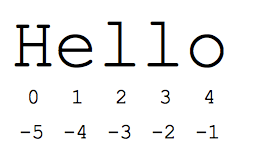
\includegraphics{hello.png}
\caption{Figure 1}
\end{figure}

    \begin{itemize}
\tightlist
\item
  \textbf{String slicing} String slicing is the python method to
  retrieve a substring of a given string. As a casual indexing, we can
  use square brackets to slice a string as follows:
\end{itemize}

\textbf{str.{[}start: stop: step{]}}

\textbf{start}: the position of the first character to retrieve.

\textbf{stop}: the position of the last character to retrieve.

\textbf{step}: how many steps to take.

    \begin{Verbatim}[commandchars=\\\{\}]
{\color{incolor}In [{\color{incolor}40}]:} \PY{n+nb}{print}\PY{p}{(}\PY{l+s+s1}{\PYZsq{}}\PY{l+s+s1}{a is:}\PY{l+s+s1}{\PYZsq{}}\PY{p}{,}\PY{n}{a}\PY{p}{)}
         
         \PY{n+nb}{print}\PY{p}{(}\PY{l+s+s1}{\PYZsq{}}\PY{l+s+s1}{starts from the third char to seventh char.}\PY{l+s+s1}{\PYZsq{}}\PY{p}{)}
         \PY{n+nb}{print}\PY{p}{(}\PY{n}{a}\PY{p}{[}\PY{l+m+mi}{2}\PY{p}{:}\PY{l+m+mi}{6}\PY{p}{]}\PY{p}{)}
         
         \PY{n+nb}{print}\PY{p}{(}\PY{l+s+s1}{\PYZsq{}}\PY{l+s+s1}{starts from the second char to seventh char stepping two chars at a time.}\PY{l+s+s1}{\PYZsq{}}\PY{p}{)}
         \PY{n+nb}{print}\PY{p}{(}\PY{n}{a}\PY{p}{[}\PY{l+m+mi}{2}\PY{p}{:}\PY{l+m+mi}{6}\PY{p}{:}\PY{l+m+mi}{2}\PY{p}{]}\PY{p}{)}
         
         \PY{c+c1}{\PYZsh{}this will return the whole string :)}
         \PY{n+nb}{print}\PY{p}{(}\PY{l+s+s2}{\PYZdq{}}\PY{l+s+s2}{the whole }\PY{l+s+s2}{\PYZsq{}}\PY{l+s+s2}{a}\PY{l+s+s2}{\PYZsq{}}\PY{l+s+s2}{ string is:}\PY{l+s+s2}{\PYZdq{}}\PY{p}{,} \PY{n}{a}\PY{p}{[}\PY{l+m+mi}{0}\PY{p}{:}\PY{n+nb}{len}\PY{p}{(}\PY{n}{a}\PY{p}{)}\PY{p}{]}\PY{p}{)}
\end{Verbatim}


    \begin{Verbatim}[commandchars=\\\{\}]
a is: this is a string
starts from the third char to seventh char.
is i
starts from the second char to seventh char stepping two chars at a time.
i 
the whole 'a' string is: this is a string

    \end{Verbatim}

    \begin{itemize}
\tightlist
\item
  \textbf{More on slicing}
\end{itemize}

    Many things we can do with strings. - we can leave indexes empty so that
python can use the default values. (i.e {[} : : {]}). - defalut value
for \textbf{start} is 0. - default value for \textbf{stop} is
\emph{len()}. - default value for \textbf{step} is 1. - negative indexes
are allowed. - {[} : : -1{]} will flip the defaults to: {[}-1:
-(len()+1):-1{]}. Simply, it will reverse the string because it will
start from the last element up to the first one. - If negative numbers
are used in the \textbf{step}, then \textbf{start} must be greater than
stop and the other way around for positive numbers.

    \begin{Verbatim}[commandchars=\\\{\}]
{\color{incolor}In [{\color{incolor}43}]:} \PY{n+nb}{print}\PY{p}{(}\PY{l+s+s2}{\PYZdq{}}\PY{l+s+s2}{this is }\PY{l+s+s2}{\PYZsq{}}\PY{l+s+s2}{a}\PY{l+s+s2}{\PYZsq{}}\PY{l+s+s2}{ string:}\PY{l+s+s2}{\PYZdq{}}\PY{p}{,} \PY{n}{a}\PY{p}{)}
         
         \PY{c+c1}{\PYZsh{} using default values will return the whole string:}
         \PY{n+nb}{print}\PY{p}{(}\PY{n}{a}\PY{p}{[}\PY{p}{:}\PY{p}{:}\PY{p}{]}\PY{p}{)}
         
         \PY{c+c1}{\PYZsh{} reverse the string:}
         \PY{n+nb}{print}\PY{p}{(}\PY{n}{a}\PY{p}{[}\PY{p}{:}\PY{p}{:}\PY{o}{\PYZhy{}}\PY{l+m+mi}{1}\PY{p}{]}\PY{p}{)}
\end{Verbatim}


    \begin{Verbatim}[commandchars=\\\{\}]
this is 'a' string: this is a string
this is a string
gnirts a si siht

    \end{Verbatim}

    \begin{itemize}
\tightlist
\item
  \textbf{Split}
\end{itemize}

    You can split a given string into a list of strings based on a given
delimiter. Suppose that I want to get all the words separated by a space
from a string, then this function is useful. Do not worry about the word
\texttt{list} will talk about it later.

    \begin{Verbatim}[commandchars=\\\{\}]
{\color{incolor}In [{\color{incolor}118}]:} \PY{n}{a} \PY{o}{=} \PY{l+s+s2}{\PYZdq{}}\PY{l+s+s2}{This is a string!!}\PY{l+s+s2}{\PYZdq{}}
          \PY{c+c1}{\PYZsh{} if there is nothing passed to the funtion,}
          \PY{c+c1}{\PYZsh{}then the default is the white sapce.}
          \PY{n+nb}{print}\PY{p}{(}\PY{n}{a}\PY{o}{.}\PY{n}{split}\PY{p}{(}\PY{p}{)}\PY{p}{)}
\end{Verbatim}


    \begin{Verbatim}[commandchars=\\\{\}]
['This', 'is', 'a', 'string!!']

    \end{Verbatim}

    \begin{itemize}
\tightlist
\item
  \textbf{join}
\end{itemize}

    Join() function is the opposite of the split function. It takes a list
of strings and add them up to one string. We can use a given string as a
connector. Look at the following code:

    \begin{Verbatim}[commandchars=\\\{\}]
{\color{incolor}In [{\color{incolor}122}]:} \PY{n}{a}\PY{o}{=}\PY{l+s+s2}{\PYZdq{}}\PY{l+s+s2}{this is}\PY{l+s+s2}{\PYZdq{}}
          \PY{n}{b}\PY{o}{=}\PY{l+s+s2}{\PYZdq{}}\PY{l+s+s2}{a string}\PY{l+s+s2}{\PYZdq{}}
          \PY{c+c1}{\PYZsh{} join the two strings with comma in between}
          \PY{n+nb}{print}\PY{p}{(}\PY{l+s+s2}{\PYZdq{}}\PY{l+s+s2}{, }\PY{l+s+s2}{\PYZdq{}}\PY{o}{.}\PY{n}{join}\PY{p}{(}\PY{p}{[}\PY{n}{a}\PY{p}{,}\PY{n}{b}\PY{p}{]}\PY{p}{)}\PY{p}{)}
\end{Verbatim}


    \begin{Verbatim}[commandchars=\\\{\}]
this is, a string

    \end{Verbatim}

    \paragraph{More python string
functions.}\label{more-python-string-functions.}

    This section, will talk about general strings functions. The description
of each method is given within the code block in the following coding
paragraph.

    \begin{Verbatim}[commandchars=\\\{\}]
{\color{incolor}In [{\color{incolor}89}]:} \PY{n}{a} \PY{o}{=} \PY{l+s+s2}{\PYZdq{}}\PY{l+s+s2}{This is a string}\PY{l+s+s2}{\PYZdq{}}
         
         \PY{c+c1}{\PYZsh{} the following functions are self\PYZhy{}descriptive functions.}
         \PY{n}{a} \PY{o}{=} \PY{n}{a}\PY{o}{.}\PY{n}{upper}\PY{p}{(}\PY{p}{)}
         \PY{n+nb}{print}\PY{p}{(}\PY{l+s+s2}{\PYZdq{}}\PY{l+s+s2}{1:}\PY{l+s+s2}{\PYZdq{}}\PY{p}{,}\PY{n}{a}\PY{p}{)}
         
         \PY{n}{a} \PY{o}{=} \PY{n}{a}\PY{o}{.}\PY{n}{lower}\PY{p}{(}\PY{p}{)}
         \PY{n+nb}{print}\PY{p}{(}\PY{l+s+s2}{\PYZdq{}}\PY{l+s+s2}{2:}\PY{l+s+s2}{\PYZdq{}}\PY{p}{,}\PY{n}{a}\PY{p}{)}
         
         
         \PY{c+c1}{\PYZsh{} the following functions will test the given string according to their namings.}
         
         \PY{c+c1}{\PYZsh{}This function test whether a string is all alphabets.}
         \PY{c+c1}{\PYZsh{}Spaces and !! will cause the function to return False.}
         \PY{n+nb}{print}\PY{p}{(}\PY{l+s+s2}{\PYZdq{}}\PY{l+s+s2}{3:}\PY{l+s+s2}{\PYZdq{}}\PY{p}{,}\PY{n}{a}\PY{o}{.}\PY{n}{isalpha}\PY{p}{(}\PY{p}{)}\PY{p}{)}
         
         \PY{c+c1}{\PYZsh{}By the way, You can define a string on the fly and test it against this function.}
         \PY{c+c1}{\PYZsh{}Look at this code:}
         \PY{n+nb}{print}\PY{p}{(}\PY{l+s+s2}{\PYZdq{}}\PY{l+s+s2}{4:}\PY{l+s+s2}{\PYZdq{}}\PY{p}{,}\PY{l+s+s2}{\PYZdq{}}\PY{l+s+s2}{thisstringisallalphabetics}\PY{l+s+s2}{\PYZdq{}}\PY{o}{.}\PY{n}{isalpha}\PY{p}{(}\PY{p}{)}\PY{p}{)}
         
         \PY{c+c1}{\PYZsh{}tests for digits:}
         \PY{n+nb}{print}\PY{p}{(}\PY{l+s+s2}{\PYZdq{}}\PY{l+s+s2}{5:}\PY{l+s+s2}{\PYZdq{}}\PY{p}{,}\PY{n}{a}\PY{o}{.}\PY{n}{isdigit}\PY{p}{(}\PY{p}{)}\PY{p}{)}
         \PY{n+nb}{print}\PY{p}{(}\PY{l+s+s2}{\PYZdq{}}\PY{l+s+s2}{6:}\PY{l+s+s2}{\PYZdq{}}\PY{p}{,}\PY{l+s+s2}{\PYZdq{}}\PY{l+s+s2}{123456789}\PY{l+s+s2}{\PYZdq{}}\PY{o}{.}\PY{n}{isdigit}\PY{p}{(}\PY{p}{)}\PY{p}{)}
         
         \PY{c+c1}{\PYZsh{}tests for space:}
         \PY{n+nb}{print}\PY{p}{(}\PY{l+s+s2}{\PYZdq{}}\PY{l+s+s2}{7:}\PY{l+s+s2}{\PYZdq{}}\PY{p}{,}\PY{n}{a}\PY{o}{.}\PY{n}{isspace}\PY{p}{(}\PY{p}{)}\PY{p}{)}
         \PY{n+nb}{print}\PY{p}{(}\PY{l+s+s2}{\PYZdq{}}\PY{l+s+s2}{8:}\PY{l+s+s2}{\PYZdq{}}\PY{p}{,}\PY{l+s+s2}{\PYZdq{}}\PY{l+s+s2}{  }\PY{l+s+s2}{\PYZdq{}}\PY{o}{.}\PY{n}{isspace}\PY{p}{(}\PY{p}{)}\PY{p}{)}
         
         
         \PY{c+c1}{\PYZsh{} this function will search a string for a given substring.}
         \PY{c+c1}{\PYZsh{} it returns the index of teh first occurance.}
         \PY{n+nb}{print}\PY{p}{(}\PY{l+s+s2}{\PYZdq{}}\PY{l+s+s2}{9:}\PY{l+s+s2}{\PYZdq{}}\PY{p}{,}\PY{n}{a}\PY{o}{.}\PY{n}{find}\PY{p}{(}\PY{l+s+s2}{\PYZdq{}}\PY{l+s+s2}{is}\PY{l+s+s2}{\PYZdq{}}\PY{p}{)}\PY{p}{)}
         
         \PY{c+c1}{\PYZsh{} this function will replace a given substring with another substring.}
         
         \PY{n}{a} \PY{o}{=} \PY{n}{a}\PY{o}{.}\PY{n}{replace}\PY{p}{(}\PY{l+s+s2}{\PYZdq{}}\PY{l+s+s2}{string}\PY{l+s+s2}{\PYZdq{}}\PY{p}{,}\PY{l+s+s2}{\PYZdq{}}\PY{l+s+s2}{nicer string!!}\PY{l+s+s2}{\PYZdq{}}\PY{p}{)}
         \PY{n+nb}{print}\PY{p}{(}\PY{l+s+s2}{\PYZdq{}}\PY{l+s+s2}{10:}\PY{l+s+s2}{\PYZdq{}}\PY{p}{,}\PY{n}{a}\PY{p}{)}
         
         \PY{c+c1}{\PYZsh{}}
\end{Verbatim}


    \begin{Verbatim}[commandchars=\\\{\}]
1: THIS IS A STRING
2: this is a string
3: False
4: True
5: False
6: True
7: False
8: True
9: 2
10: this is a nicer string!!

    \end{Verbatim}

    And by this ends the String section.

    \subsection{Python Operators}\label{python-operators}

    Operators are special characters with specific functionalities. There
are different types of operands. The following lists will show many
operands of different kinds.

    I just copied and pasted these lists from this good sources:
https://www.geeksforgeeks.org/basic-operators-python/

    \textbf{Operator Description Syntax} \_\_\_\_\_\_\_\_

\begin{verbatim}
- Arithmetic Operators.
\end{verbatim}

\begin{itemize}
\item
  {[}+{]} Addition: adds two operands x + y
\item
  {[}-{]} Subtraction: subtracts two operands x - y
\item
  {[}*{]} Multiplication: multiplies two operands x * y
\item
  {[}/{]} Division (float): divides the first operand by the second x /
  y
\item ~
  \subsection{{[}//{]} Division (floor): divides the first operand by
  the second x //
  y}\label{division-floor-divides-the-first-operand-by-the-second-x-y}

  \begin{itemize}
  \tightlist
  \item
    Relational Operators.
  \end{itemize}
\item
  {[}\textgreater{}{]} Greater than: True if left operand is greater
  than the right x \textgreater{} y
\item
  {[}\textless{}{]} Less than: True if left operand is less than the
  right x \textless{} y
\item
  {[}=={]} Equal to: True if both operands are equal x == y
\item
  {[}!={]} Not equal to - True if operands are not equal x != y
\item
  {[}\textgreater{}={]} Greater than or equal to: True if left operand
  is greater than or equal to the right x \textgreater{}= y
\item ~
  \subsection{{[}\textless{}={]} Less than or equal to: True if left
  operand is less than or equal to the right x \textless{}=
  y}\label{less-than-or-equal-to-true-if-left-operand-is-less-than-or-equal-to-the-right-x-y}

  \begin{itemize}
  \tightlist
  \item
    Logical Operators
  \end{itemize}
\item
  and Logical AND: True if both the operands are true x and y
\item
  or Logical OR: True if either of the operands is true x or y
\item ~
  \subsection{not Logical NOT: True if operand is false not
  x}\label{not-logical-not-true-if-operand-is-false-not-x}

  \begin{itemize}
  \tightlist
  \item
    Assignment Operators
  \end{itemize}
\item
  = Assign value of right side of expression to left side operand x = y
  + z
\item
  += Add AND: Add right side operand with left side operand and then
  assign to left operand a+=b a=a+b
\item
  -= Subtract AND: Subtract right operand from left operand and then
  assign to left operand a-=b a=a-b
\item
  \emph{= Multiply AND: Multiply right operand with left operand and
  then assign to left operand a}=b a=a*b
\item
  /= Divide AND: Divide left operand with right operand and then assign
  to left operand a/=b a=a/b
\item
  \%= Modulus AND: Takes modulus using left and right operands and
  assign result to left operand a\%=b a=a\%b
\item
  //= Divide(floor) AND: Divide left operand with right operand and then
  assign the value(floor) to left operand a//=b a=a//b
\item
  **= Exponent AND: Calculate exponent(raise power) value using operands
  and assign value to left operand
\end{itemize}

    \begin{Verbatim}[commandchars=\\\{\}]
{\color{incolor}In [{\color{incolor}130}]:} \PY{c+c1}{\PYZsh{} Examples of Arithmetic Operator}
          \PY{n}{a} \PY{o}{=} \PY{l+m+mi}{9}
          \PY{n}{b} \PY{o}{=} \PY{l+m+mi}{4}
           
          \PY{c+c1}{\PYZsh{} Addition of numbers}
          \PY{n}{add} \PY{o}{=} \PY{n}{a} \PY{o}{+} \PY{n}{b}
          \PY{c+c1}{\PYZsh{} Subtraction of numbers }
          \PY{n}{sub} \PY{o}{=} \PY{n}{a} \PY{o}{\PYZhy{}} \PY{n}{b}
          \PY{c+c1}{\PYZsh{} Multiplication of number }
          \PY{n}{mul} \PY{o}{=} \PY{n}{a} \PY{o}{*} \PY{n}{b}
          \PY{c+c1}{\PYZsh{} Division(float) of number }
          \PY{n}{div1} \PY{o}{=} \PY{n}{a} \PY{o}{/} \PY{n}{b}
          \PY{c+c1}{\PYZsh{} Division(floor) of number }
          \PY{n}{div2} \PY{o}{=} \PY{n}{a} \PY{o}{/}\PY{o}{/} \PY{n}{b}
          \PY{c+c1}{\PYZsh{} Modulo of both number}
          \PY{n}{mod} \PY{o}{=} \PY{n}{a} \PY{o}{\PYZpc{}} \PY{n}{b}
           
          \PY{c+c1}{\PYZsh{} print results}
          \PY{n+nb}{print}\PY{p}{(}\PY{n}{add}\PY{p}{)}
          \PY{n+nb}{print}\PY{p}{(}\PY{n}{sub}\PY{p}{)}
          \PY{n+nb}{print}\PY{p}{(}\PY{n}{mul}\PY{p}{)}
          \PY{n+nb}{print}\PY{p}{(}\PY{n}{div1}\PY{p}{)}
          \PY{n+nb}{print}\PY{p}{(}\PY{n}{div2}\PY{p}{)}
          \PY{n+nb}{print}\PY{p}{(}\PY{n}{mod}\PY{p}{)}
          
          
          \PY{c+c1}{\PYZsh{} Examples of Relational Operators}
          \PY{n}{a} \PY{o}{=} \PY{l+m+mi}{13}
          \PY{n}{b} \PY{o}{=} \PY{l+m+mi}{33}
           
          \PY{c+c1}{\PYZsh{} a \PYZgt{} b is False}
          \PY{n+nb}{print}\PY{p}{(}\PY{n}{a} \PY{o}{\PYZgt{}} \PY{n}{b}\PY{p}{)}
           
          \PY{c+c1}{\PYZsh{} a \PYZlt{} b is True}
          \PY{n+nb}{print}\PY{p}{(}\PY{n}{a} \PY{o}{\PYZlt{}} \PY{n}{b}\PY{p}{)}
           
          \PY{c+c1}{\PYZsh{} a == b is False}
          \PY{n+nb}{print}\PY{p}{(}\PY{n}{a} \PY{o}{==} \PY{n}{b}\PY{p}{)}
           
          \PY{c+c1}{\PYZsh{} a != b is True}
          \PY{n+nb}{print}\PY{p}{(}\PY{n}{a} \PY{o}{!=} \PY{n}{b}\PY{p}{)}
           
          \PY{c+c1}{\PYZsh{} a \PYZgt{}= b is False}
          \PY{n+nb}{print}\PY{p}{(}\PY{n}{a} \PY{o}{\PYZgt{}}\PY{o}{=} \PY{n}{b}\PY{p}{)}
           
          \PY{c+c1}{\PYZsh{} a \PYZlt{}= b is True}
          \PY{n+nb}{print}\PY{p}{(}\PY{n}{a} \PY{o}{\PYZlt{}}\PY{o}{=} \PY{n}{b}\PY{p}{)}
          
          
          \PY{c+c1}{\PYZsh{} Examples of Logical Operator}
          \PY{n}{a} \PY{o}{=} \PY{k+kc}{True}
          \PY{n}{b} \PY{o}{=} \PY{k+kc}{False}
           
          \PY{c+c1}{\PYZsh{} Print a and b is False}
          \PY{n+nb}{print}\PY{p}{(}\PY{n}{a} \PY{o+ow}{and} \PY{n}{b}\PY{p}{)}
           
          \PY{c+c1}{\PYZsh{} Print a or b is True}
          \PY{n+nb}{print}\PY{p}{(}\PY{n}{a} \PY{o+ow}{or} \PY{n}{b}\PY{p}{)}
           
          \PY{c+c1}{\PYZsh{} Print not a is False}
          \PY{n+nb}{print}\PY{p}{(}\PY{o+ow}{not} \PY{n}{a}\PY{p}{)}
\end{Verbatim}


    \begin{Verbatim}[commandchars=\\\{\}]
13
5
36
2.25
2
1
False
True
False
True
False
True
False
True
False

    \end{Verbatim}

    \subsection{Python Data Structures}\label{python-data-structures}

    The previous data types are so useful. They are used to hold the data we
need to process. However, they are not enough. What about having a dozen
of data? defining variables for each is redundant or even ridiculous!
That is why python, as many other languages, provides data structures.

    \subsubsection{Lists}\label{lists}

    Lists are one of the simplest data types. You can think of it as a
sequence of elements. In that context, we can say that strings are
special type of lists as they are just a sequence of characters. In
fact, both of them "strings and lists" shares many properties and
functions. \textbf{keep in mind that lists should contain elements of
the same type!!}

    \paragraph{Playing with lists.}\label{playing-with-lists.}

    \begin{Verbatim}[commandchars=\\\{\}]
{\color{incolor}In [{\color{incolor}191}]:} \PY{c+c1}{\PYZsh{} to define a new list:}
          \PY{n}{mylist} \PY{o}{=} \PY{p}{[}\PY{p}{]}
          
          \PY{c+c1}{\PYZsh{} you can also say:}
          \PY{n}{mylist2} \PY{o}{=} \PY{p}{[}\PY{l+m+mi}{1}\PY{p}{,}\PY{l+m+mi}{2}\PY{p}{,}\PY{l+m+mi}{3}\PY{p}{,}\PY{l+m+mi}{4}\PY{p}{,}\PY{l+m+mi}{5}\PY{p}{,}\PY{l+m+mi}{6}\PY{p}{,}\PY{l+m+mi}{7}\PY{p}{,}\PY{l+m+mi}{8}\PY{p}{,}\PY{l+m+mi}{9}\PY{p}{]}
          
          \PY{c+c1}{\PYZsh{} add item to a list:}
          \PY{n}{mylist}\PY{o}{.}\PY{n}{append}\PY{p}{(}\PY{l+m+mi}{0}\PY{p}{)}
          \PY{n+nb}{print}\PY{p}{(}\PY{l+s+s2}{\PYZdq{}}\PY{l+s+s2}{1: mylilst:}\PY{l+s+s2}{\PYZdq{}}\PY{p}{,}\PY{n}{mylist}\PY{p}{)}
          
          \PY{c+c1}{\PYZsh{}add list to list:}
          \PY{n}{mylist}\PY{o}{.}\PY{n}{extend}\PY{p}{(}\PY{n}{mylist2}\PY{p}{)}
          \PY{n+nb}{print}\PY{p}{(}\PY{l+s+s2}{\PYZdq{}}\PY{l+s+s2}{2: mylist:}\PY{l+s+s2}{\PYZdq{}}\PY{p}{,} \PY{n}{mylist}\PY{p}{)}
          \PY{c+c1}{\PYZsh{} you can also use this shortcut:}
          \PY{c+c1}{\PYZsh{}mylist += mylist2}
          
          \PY{c+c1}{\PYZsh{}you can insert items to any index:}
          \PY{n}{mylist}\PY{o}{.}\PY{n}{insert}\PY{p}{(}\PY{l+m+mi}{7}\PY{p}{,}\PY{l+m+mi}{7}\PY{p}{)}
          \PY{n+nb}{print}\PY{p}{(}\PY{l+s+s2}{\PYZdq{}}\PY{l+s+s2}{3: mylist:}\PY{l+s+s2}{\PYZdq{}}\PY{p}{,} \PY{n}{mylist}\PY{p}{)}
          
          \PY{c+c1}{\PYZsh{}Remove the first item from the list whose value is x.}
          \PY{n}{mylist}\PY{o}{.}\PY{n}{remove}\PY{p}{(}\PY{l+m+mi}{7}\PY{p}{)}
          \PY{n+nb}{print}\PY{p}{(}\PY{l+s+s2}{\PYZdq{}}\PY{l+s+s2}{4: mylist}\PY{l+s+s2}{\PYZdq{}}\PY{p}{,}\PY{n}{mylist}\PY{p}{)}
          \PY{c+c1}{\PYZsh{}It is an error if there is no such item.}
          \PY{c+c1}{\PYZsh{} the following line will produce an error:}
          \PY{c+c1}{\PYZsh{}mylist.remove(10)}
          
          \PY{c+c1}{\PYZsh{} or you can delete element at a given index:}
          \PY{k}{del} \PY{n}{mylist}\PY{p}{[}\PY{l+m+mi}{0}\PY{p}{]}
          \PY{n+nb}{print}\PY{p}{(}\PY{l+s+s2}{\PYZdq{}}\PY{l+s+s2}{5: mylist:}\PY{l+s+s2}{\PYZdq{}}\PY{p}{,}\PY{n}{mylist}\PY{p}{)}
          
          \PY{c+c1}{\PYZsh{} you can use pop() function to do the same thing.}
          \PY{c+c1}{\PYZsh{} However, passing no index to pop() will delete the last element of the array.}
          \PY{n}{mylist}\PY{o}{.}\PY{n}{pop}\PY{p}{(}\PY{p}{)}
          \PY{n+nb}{print}\PY{p}{(}\PY{l+s+s2}{\PYZdq{}}\PY{l+s+s2}{6: mylist:}\PY{l+s+s2}{\PYZdq{}}\PY{p}{,} \PY{n}{mylist}\PY{p}{)}
          \PY{n}{mylist}\PY{o}{.}\PY{n}{pop}\PY{p}{(}\PY{l+m+mi}{0}\PY{p}{)}
          \PY{n+nb}{print}\PY{p}{(}\PY{l+s+s2}{\PYZdq{}}\PY{l+s+s2}{7: mylist:}\PY{l+s+s2}{\PYZdq{}}\PY{p}{,}\PY{n}{mylist}\PY{p}{)}
          
          
          \PY{c+c1}{\PYZsh{} to clear the list \PYZdq{}remove all elements at once\PYZdq{}:}
          \PY{n}{mylist}\PY{o}{.}\PY{n}{clear}\PY{p}{(}\PY{p}{)}
          \PY{n+nb}{print}\PY{p}{(}\PY{l+s+s2}{\PYZdq{}}\PY{l+s+s2}{8: mylist:}\PY{l+s+s2}{\PYZdq{}}\PY{p}{,}\PY{n}{mylist}\PY{p}{)}
          \PY{c+c1}{\PYZsh{} let us return our list back for further manipulations:}
          \PY{n}{mylist} \PY{o}{=} \PY{p}{[}\PY{l+m+mi}{0}\PY{p}{,}\PY{l+m+mi}{1}\PY{p}{,}\PY{l+m+mi}{2}\PY{p}{,}\PY{l+m+mi}{3}\PY{p}{,}\PY{l+m+mi}{4}\PY{p}{,}\PY{l+m+mi}{5}\PY{p}{,}\PY{l+m+mi}{6}\PY{p}{,}\PY{l+m+mi}{7}\PY{p}{,}\PY{l+m+mi}{8}\PY{p}{,}\PY{l+m+mi}{9}\PY{p}{]}
          
          \PY{c+c1}{\PYZsh{} as we have done with string, we can index lists as well.}
          \PY{c+c1}{\PYZsh{} this will retrive elements in the odd indexes:}
          \PY{n}{sublist} \PY{o}{=} \PY{n}{mylist}\PY{p}{[}\PY{l+m+mi}{1}\PY{p}{:}\PY{p}{:}\PY{l+m+mi}{2}\PY{p}{]}
          \PY{n+nb}{print}\PY{p}{(}\PY{l+s+s2}{\PYZdq{}}\PY{l+s+s2}{9: sublist:}\PY{l+s+s2}{\PYZdq{}}\PY{p}{,}\PY{n}{sublist}\PY{p}{)}
          \PY{c+c1}{\PYZsh{}negative indexes applies to lists as well. BUT REVERSED:}
          \PY{n}{sublist} \PY{o}{=} \PY{n}{mylist}\PY{p}{[}\PY{l+m+mi}{5}\PY{p}{:}\PY{l+m+mi}{0}\PY{p}{:}\PY{o}{\PYZhy{}}\PY{l+m+mi}{1}\PY{p}{]}
          \PY{n+nb}{print}\PY{p}{(}\PY{l+s+s2}{\PYZdq{}}\PY{l+s+s2}{10: the first five elements reversed:}\PY{l+s+s2}{\PYZdq{}}\PY{p}{,}\PY{n}{sublist}\PY{p}{)}
          
          \PY{c+c1}{\PYZsh{} you can reverse the list as follows:}
          \PY{n}{mylist}\PY{o}{.}\PY{n}{reverse}\PY{p}{(}\PY{p}{)}
          \PY{n+nb}{print}\PY{p}{(}\PY{l+s+s2}{\PYZdq{}}\PY{l+s+s2}{11: mylist:}\PY{l+s+s2}{\PYZdq{}}\PY{p}{,} \PY{n}{mylist}\PY{p}{)}
          
          \PY{c+c1}{\PYZsh{}you can sort the list as follows:}
          \PY{n}{mylist}\PY{o}{.}\PY{n}{sort}\PY{p}{(}\PY{p}{)}
          \PY{n+nb}{print}\PY{p}{(}\PY{l+s+s2}{\PYZdq{}}\PY{l+s+s2}{12: mylist:}\PY{l+s+s2}{\PYZdq{}}\PY{p}{,} \PY{n}{mylist}\PY{p}{)}
          \PY{c+c1}{\PYZsh{} you can also sort with reverse as follows:}
          \PY{c+c1}{\PYZsh{}mylist.sort(reverse=True)}
          
          \PY{c+c1}{\PYZsh{} you can get the number an elements is repeated in a list:}
          \PY{n+nb}{print}\PY{p}{(}\PY{l+s+s2}{\PYZdq{}}\PY{l+s+s2}{13: number of 5}\PY{l+s+s2}{\PYZsq{}}\PY{l+s+s2}{s:}\PY{l+s+s2}{\PYZdq{}}\PY{p}{,}\PY{n}{mylist}\PY{o}{.}\PY{n}{count}\PY{p}{(}\PY{l+m+mi}{5}\PY{p}{)}\PY{p}{)}
          
          \PY{c+c1}{\PYZsh{} len() function can be used to get the number of elements:}
          \PY{n+nb}{print}\PY{p}{(}\PY{l+s+s2}{\PYZdq{}}\PY{l+s+s2}{14: number of elements in mylist:}\PY{l+s+s2}{\PYZdq{}}\PY{p}{,}\PY{n+nb}{len}\PY{p}{(}\PY{n}{mylist}\PY{p}{)}\PY{p}{)}
          
          \PY{c+c1}{\PYZsh{} you can retrive the index of any element:}
          \PY{n+nb}{print}\PY{p}{(}\PY{l+s+s2}{\PYZdq{}}\PY{l+s+s2}{15: index of 5:}\PY{l+s+s2}{\PYZdq{}}\PY{p}{,} \PY{n}{mylist}\PY{o}{.}\PY{n}{index}\PY{p}{(}\PY{l+m+mi}{5}\PY{p}{)}\PY{p}{)}
          
          \PY{c+c1}{\PYZsh{}\PYZhy{}\PYZhy{}\PYZhy{}\PYZhy{}\PYZhy{}\PYZhy{}\PYZhy{}\PYZhy{}\PYZhy{}\PYZhy{}\PYZhy{}\PYZhy{}\PYZhy{}\PYZhy{}\PYZhy{}\PYZhy{}\PYZhy{}\PYZhy{}\PYZhy{}\PYZhy{}\PYZhy{}\PYZhy{}\PYZhy{}\PYZhy{}\PYZhy{}\PYZhy{}\PYZhy{}\PYZhy{}\PYZhy{}\PYZhy{}\PYZhy{}\PYZhy{}\PYZhy{}\PYZhy{}\PYZhy{}\PYZhy{}\PYZhy{}\PYZhy{}\PYZhy{}\PYZhy{}\PYZhy{}\PYZhy{}\PYZhy{}\PYZhy{}\PYZhy{}\PYZhy{}\PYZhy{}\PYZhy{}\PYZhy{}\PYZhy{}\PYZhy{}\PYZhy{}\PYZhy{}\PYZhy{}\PYZhy{}\PYZhy{}\PYZhy{}\PYZhy{}\PYZhy{}\PYZhy{}\PYZhy{}}
          \PY{c+c1}{\PYZsh{} The following methods are only applicable for numeric types:}
          \PY{c+c1}{\PYZsh{}\PYZhy{}\PYZhy{}\PYZhy{}\PYZhy{}\PYZhy{}\PYZhy{}\PYZhy{}\PYZhy{}\PYZhy{}\PYZhy{}\PYZhy{}\PYZhy{}\PYZhy{}\PYZhy{}\PYZhy{}\PYZhy{}\PYZhy{}\PYZhy{}\PYZhy{}\PYZhy{}\PYZhy{}\PYZhy{}\PYZhy{}\PYZhy{}\PYZhy{}\PYZhy{}\PYZhy{}\PYZhy{}\PYZhy{}\PYZhy{}\PYZhy{}\PYZhy{}\PYZhy{}\PYZhy{}\PYZhy{}\PYZhy{}\PYZhy{}\PYZhy{}\PYZhy{}\PYZhy{}\PYZhy{}\PYZhy{}\PYZhy{}\PYZhy{}\PYZhy{}\PYZhy{}\PYZhy{}\PYZhy{}\PYZhy{}\PYZhy{}\PYZhy{}\PYZhy{}\PYZhy{}\PYZhy{}\PYZhy{}\PYZhy{}\PYZhy{}\PYZhy{}\PYZhy{}\PYZhy{}\PYZhy{}}
          \PY{c+c1}{\PYZsh{} sum a list:}
          \PY{n+nb}{print}\PY{p}{(}\PY{l+s+s2}{\PYZdq{}}\PY{l+s+s2}{16: sum of mylist elements:}\PY{l+s+s2}{\PYZdq{}}\PY{p}{,}\PY{n+nb}{sum}\PY{p}{(}\PY{n}{mylist}\PY{p}{)}\PY{p}{)}
          
          \PY{c+c1}{\PYZsh{} max of list:}
          \PY{n+nb}{print}\PY{p}{(}\PY{l+s+s2}{\PYZdq{}}\PY{l+s+s2}{17: max of mylist:}\PY{l+s+s2}{\PYZdq{}}\PY{p}{,} \PY{n+nb}{max}\PY{p}{(}\PY{n}{mylist}\PY{p}{)}\PY{p}{)}
          
          \PY{c+c1}{\PYZsh{} min of list:}
          \PY{n+nb}{print}\PY{p}{(}\PY{l+s+s2}{\PYZdq{}}\PY{l+s+s2}{18: min of mylist:}\PY{l+s+s2}{\PYZdq{}}\PY{p}{,} \PY{n+nb}{min}\PY{p}{(}\PY{n}{mylist}\PY{p}{)}\PY{p}{)}
\end{Verbatim}


    \begin{Verbatim}[commandchars=\\\{\}]
1: mylilst: [0]
2: mylist: [0, 1, 2, 3, 4, 5, 6, 7, 8, 9]
3: mylist: [0, 1, 2, 3, 4, 5, 6, 7, 7, 8, 9]
4: mylist [0, 1, 2, 3, 4, 5, 6, 7, 8, 9]
5: mylist: [1, 2, 3, 4, 5, 6, 7, 8, 9]
6: mylist: [1, 2, 3, 4, 5, 6, 7, 8]
7: mylist: [2, 3, 4, 5, 6, 7, 8]
8: mylist: []
9: sublist: [1, 3, 5, 7, 9]
10: the first five elements reversed: [5, 4, 3, 2, 1]
11: mylist: [9, 8, 7, 6, 5, 4, 3, 2, 1, 0]
12: mylist: [0, 1, 2, 3, 4, 5, 6, 7, 8, 9]
13: number of 5's: 1
14: number of elements in mylist: 10
15: index of 5: 5
16: sum of mylist elements: 45
17: max of mylist: 9
18: min of mylist: 0

    \end{Verbatim}

    \begin{Verbatim}[commandchars=\\\{\}]
{\color{incolor}In [{\color{incolor}192}]:} \PY{c+c1}{\PYZsh{} range function usage}
          \PY{c+c1}{\PYZsh{} get list from 0,10}
          \PY{n+nb}{print}\PY{p}{(}\PY{n+nb}{range}\PY{p}{(}\PY{l+m+mi}{10}\PY{p}{)}\PY{p}{)}
\end{Verbatim}


    \begin{Verbatim}[commandchars=\\\{\}]
range(0, 10)

    \end{Verbatim}

    \subsubsection{Dictionaries}\label{dictionaries}

    It is a useful data structure. The different between lists and
dictionaries is that lists are indexed by integers while dictionaries
are indexed by sort of keys!

    \paragraph{Playing with dictionaries}\label{playing-with-dictionaries}

    \begin{Verbatim}[commandchars=\\\{\}]
{\color{incolor}In [{\color{incolor}193}]:} \PY{c+c1}{\PYZsh{} initialize a dictionary:}
          \PY{n+nb}{dict} \PY{o}{=} \PY{p}{\PYZob{}}\PY{l+s+s1}{\PYZsq{}}\PY{l+s+s1}{name}\PY{l+s+s1}{\PYZsq{}}\PY{p}{:}\PY{l+s+s1}{\PYZsq{}}\PY{l+s+s1}{KFUPM}\PY{l+s+s1}{\PYZsq{}}\PY{p}{,} \PY{l+s+s1}{\PYZsq{}}\PY{l+s+s1}{age}\PY{l+s+s1}{\PYZsq{}}\PY{p}{:}\PY{l+m+mi}{55}\PY{p}{\PYZcb{}}
          \PY{n+nb}{print}\PY{p}{(}\PY{l+s+s2}{\PYZdq{}}\PY{l+s+s2}{1: dict:}\PY{l+s+s2}{\PYZdq{}}\PY{p}{,}\PY{n+nb}{dict}\PY{p}{)}
          
          \PY{c+c1}{\PYZsh{} get only keys:}
          \PY{n+nb}{print}\PY{p}{(}\PY{l+s+s2}{\PYZdq{}}\PY{l+s+s2}{2: dict keys:}\PY{l+s+s2}{\PYZdq{}}\PY{p}{,}\PY{n+nb}{dict}\PY{o}{.}\PY{n}{keys}\PY{p}{(}\PY{p}{)}\PY{p}{)}
          
          \PY{c+c1}{\PYZsh{} get only values:}
          \PY{n+nb}{print}\PY{p}{(}\PY{l+s+s2}{\PYZdq{}}\PY{l+s+s2}{3: dict values:}\PY{l+s+s2}{\PYZdq{}}\PY{p}{,} \PY{n+nb}{dict}\PY{o}{.}\PY{n}{values}\PY{p}{(}\PY{p}{)}\PY{p}{)}
          
          \PY{c+c1}{\PYZsh{} update dict:}
          \PY{n+nb}{dict}\PY{p}{[}\PY{l+s+s2}{\PYZdq{}}\PY{l+s+s2}{name}\PY{l+s+s2}{\PYZdq{}}\PY{p}{]}\PY{o}{=} \PY{l+s+s2}{\PYZdq{}}\PY{l+s+s2}{King Fahd University for Petroleum and Minerals}\PY{l+s+s2}{\PYZdq{}}
          \PY{n+nb}{print}\PY{p}{(}\PY{l+s+s2}{\PYZdq{}}\PY{l+s+s2}{4:}\PY{l+s+s2}{\PYZdq{}}\PY{p}{,}\PY{n+nb}{dict}\PY{p}{)}
          
          \PY{c+c1}{\PYZsh{} add new key\PYZhy{}value element:}
          \PY{n+nb}{dict}\PY{p}{[}\PY{l+s+s2}{\PYZdq{}}\PY{l+s+s2}{short name}\PY{l+s+s2}{\PYZdq{}}\PY{p}{]}\PY{o}{=} \PY{l+s+s2}{\PYZdq{}}\PY{l+s+s2}{KFUPM}\PY{l+s+s2}{\PYZdq{}}
          \PY{n+nb}{print}\PY{p}{(}\PY{l+s+s2}{\PYZdq{}}\PY{l+s+s2}{5:}\PY{l+s+s2}{\PYZdq{}}\PY{p}{,}\PY{n+nb}{dict}\PY{p}{)}
          
          \PY{c+c1}{\PYZsh{} delete a key:}
          \PY{n+nb}{dict}\PY{o}{.}\PY{n}{pop}\PY{p}{(}\PY{l+s+s1}{\PYZsq{}}\PY{l+s+s1}{age}\PY{l+s+s1}{\PYZsq{}}\PY{p}{,}\PY{k+kc}{None}\PY{p}{)}
          \PY{n+nb}{print}\PY{p}{(}\PY{l+s+s2}{\PYZdq{}}\PY{l+s+s2}{6:}\PY{l+s+s2}{\PYZdq{}}\PY{p}{,}\PY{n+nb}{dict}\PY{p}{)}
\end{Verbatim}


    \begin{Verbatim}[commandchars=\\\{\}]
1: dict: \{'name': 'KFUPM', 'age': 55\}
2: dict keys: dict\_keys(['name', 'age'])
3: dict values: dict\_values(['KFUPM', 55])
4: \{'name': 'King Fahd University for Petroleum and Minerals', 'age': 55\}
5: \{'name': 'King Fahd University for Petroleum and Minerals', 'age': 55, 'short name': 'KFUPM'\}
6: \{'name': 'King Fahd University for Petroleum and Minerals', 'short name': 'KFUPM'\}

    \end{Verbatim}

    \subsubsection{accessing list elements}\label{accessing-list-elements}

    You can access list elements using loops. We will talk about loops later
in details. However, we will use it here to access list elements.

    \begin{Verbatim}[commandchars=\\\{\}]
{\color{incolor}In [{\color{incolor}194}]:} \PY{c+c1}{\PYZsh{}you can access list elements as follows:}
          
          \PY{n+nb}{print}\PY{p}{(}\PY{l+s+s2}{\PYZdq{}}\PY{l+s+s2}{list elements are:}\PY{l+s+s2}{\PYZdq{}}\PY{p}{)}
          \PY{k}{for} \PY{n}{elem} \PY{o+ow}{in} \PY{n}{mylist}\PY{p}{:}
              \PY{n+nb}{print}\PY{p}{(}\PY{n}{elem}\PY{p}{,} \PY{n}{end}\PY{o}{=}\PY{l+s+s2}{\PYZdq{}}\PY{l+s+s2}{, }\PY{l+s+s2}{\PYZdq{}}\PY{p}{)}
          \PY{n+nb}{print}\PY{p}{(}\PY{p}{)}
\end{Verbatim}


    \begin{Verbatim}[commandchars=\\\{\}]
list elements are:
0, 1, 2, 3, 4, 5, 6, 7, 8, 9, 

    \end{Verbatim}

    \begin{Verbatim}[commandchars=\\\{\}]
{\color{incolor}In [{\color{incolor}197}]:} \PY{c+c1}{\PYZsh{} also, you can access list elements by index.}
          \PY{c+c1}{\PYZsh{} we will use range() function to generage iterable integers.}
          \PY{c+c1}{\PYZsh{} its usage is similar to list indexes.}
          \PY{c+c1}{\PYZsh{} range(start, stop, step) with the same default values of list inexing.}
          \PY{n+nb}{print}\PY{p}{(}\PY{l+s+s2}{\PYZdq{}}\PY{l+s+s2}{elements of range() function:}\PY{l+s+s2}{\PYZdq{}}\PY{p}{)}
          \PY{k}{for} \PY{n}{i} \PY{o+ow}{in} \PY{n+nb}{range}\PY{p}{(}\PY{l+m+mi}{10}\PY{p}{)}\PY{p}{:}
              \PY{c+c1}{\PYZsh{} let us print numbers of range function:}
              \PY{n+nb}{print}\PY{p}{(}\PY{n}{i}\PY{p}{,} \PY{n}{end}\PY{o}{=}\PY{l+s+s2}{\PYZdq{}}\PY{l+s+s2}{, }\PY{l+s+s2}{\PYZdq{}}\PY{p}{)}
          \PY{n+nb}{print}\PY{p}{(}\PY{p}{)}    
          \PY{c+c1}{\PYZsh{} now, we can access list elements as follows:}
          \PY{c+c1}{\PYZsh{} multiply each list element by 2:}
          \PY{n+nb}{print}\PY{p}{(}\PY{l+s+s2}{\PYZdq{}}\PY{l+s+s2}{doubled lists elements:}\PY{l+s+s2}{\PYZdq{}}\PY{p}{)}
          \PY{k}{for} \PY{n}{i} \PY{o+ow}{in} \PY{n+nb}{range}\PY{p}{(}\PY{n+nb}{len}\PY{p}{(}\PY{n}{mylist}\PY{p}{)}\PY{p}{)}\PY{p}{:}
              \PY{n}{mylist}\PY{p}{[}\PY{n}{i}\PY{p}{]} \PY{o}{*}\PY{o}{=} \PY{l+m+mi}{2}
          
          
          \PY{n+nb}{print}\PY{p}{(}\PY{n}{mylist}\PY{p}{)}
\end{Verbatim}


    \begin{Verbatim}[commandchars=\\\{\}]
elements of range() function:
0, 1, 2, 3, 4, 5, 6, 7, 8, 9, 
doubled lists elements:
[0, 8, 16, 24, 32, 40, 48, 56, 64, 72]

    \end{Verbatim}

    \subsection{Exercises}\label{exercises}

    \begin{Verbatim}[commandchars=\\\{\}]
{\color{incolor}In [{\color{incolor}201}]:} \PY{c+c1}{\PYZsh{} use the following line to ask some input from the user.}
          
          \PY{n}{x} \PY{o}{=} \PY{n+nb}{input}\PY{p}{(}\PY{l+s+s2}{\PYZdq{}}\PY{l+s+s2}{enter some input: }\PY{l+s+s2}{\PYZdq{}}\PY{p}{)}
          \PY{n+nb}{print}\PY{p}{(}\PY{l+s+s2}{\PYZdq{}}\PY{l+s+s2}{you entered:}\PY{l+s+s2}{\PYZdq{}}\PY{p}{,}\PY{n}{x}\PY{p}{)}
\end{Verbatim}


    \begin{Verbatim}[commandchars=\\\{\}]
enter some input: Hello world of python! :)
you entered: Hello world of python! :)

    \end{Verbatim}

    \begin{Verbatim}[commandchars=\\\{\}]
{\color{incolor}In [{\color{incolor} }]:} \PY{c+c1}{\PYZsh{} Write a Python program to remove duplicates from a list.}
        
        
        
        
        
        
        
        
        
        
        \PY{c+c1}{\PYZsh{} Write a Python program to count the number of characters (character frequency)}
        \PY{c+c1}{\PYZsh{}in a string. and write them to a dictionary}
        \PY{c+c1}{\PYZsh{}Sample String : google.com\PYZsq{}}
        \PY{c+c1}{\PYZsh{}Expected Result : \PYZob{}\PYZsq{}o\PYZsq{}: 3, \PYZsq{}g\PYZsq{}: 2, \PYZsq{}.\PYZsq{}: 1, \PYZsq{}e\PYZsq{}: 1, \PYZsq{}l\PYZsq{}: 1, \PYZsq{}m\PYZsq{}: 1, \PYZsq{}c\PYZsq{}: 1\PYZcb{}}
        
        
        
        
        
        
        
        
        
        
        
        \PY{c+c1}{\PYZsh{}Write a Python program to get a single string from two given strings.}
        \PY{c+c1}{\PYZsh{}separated by a space and swap the first two characters of each string!}
        
        
        
        
        
        
        
        
        
        
        
        
        \PY{c+c1}{\PYZsh{} Write a Python program to sum all the items in a list}
        \PY{c+c1}{\PYZsh{} DO NOT USE THE SUM() FUNCTION BUT USE IT TO COMPARE WITH YOUR RESUTS}
        
        
        
        
        
        
        
        
        \PY{c+c1}{\PYZsh{}  Write a Python program to get the largest number from a list}
        \PY{c+c1}{\PYZsh{} USE THE MAX FUANCTION ONLY TO COMPARE WITH YOUR FINDINGS}
        
        
        
        
        
        
        
        \PY{c+c1}{\PYZsh{} Write a Python program to deep\PYZhy{}copy a list.}
\end{Verbatim}


    \subsection{Resources}\label{resources}

    1- https://www.pythoncentral.io/pythons-range-function-explained/

2- https://docs.python.org/3/tutorial/datastructures.html

3- https://www.tutorialspoint.com/python/python\_loops.htm

4- https://developers.google.com/edu/python/strings


    % Add a bibliography block to the postdoc
    
    
    
    \end{document}
